% -----------------------------*- LaTeX -*------------------------------
\documentclass[UTF8]{report}
% ------------------------------------------------------------------------
% Packages
% ------------------------------------------------------------------------
\usepackage{adjustbox}
\usepackage{algorithm,algorithmicx}
\usepackage[noend]{algpseudocode}
\usepackage{amsmath,amsfonts,amssymb,bm,amsthm}%数学宏包、数学字体、数学符号、支持 \mathscr{} 字体、支持粗斜体 \bm{}、数学定理
\usepackage{bigstrut,multirow,rotating}%Excel表格自动导入latex
\usepackage{booktabs}
\usepackage{breqn}
\usepackage{caption}
\usepackage{color}%支持颜色改变
\usepackage{ctex}
\usepackage{enumitem}%自定义列表环境
\usepackage{esint}%支持多种积分算子
\usepackage{extarrows}%任意长度的箭头
\usepackage{fancyhdr}
\usepackage{fontsize}
\usepackage{fontspec}
\usepackage[body={7in, 9in},left=1in,right=1in]{geometry}
\usepackage{graphicx}%支持 \includegraphics{} 插图
\usepackage{mathrsfs}
\usepackage{mathtools}%数学宏包的重要补充
\usepackage[framemethod=TikZ]{mdframed}
\usepackage{nicefrac}
\usepackage{scribe}
\usepackage{subfigure}%插入子图
\usepackage{tikz,xcolor}%画图、画 Feynman 图
\usepackage{upgreek}%数学环境的直立希腊字母
% ------------------------------------------------------------------------
% Macros
% ------------------------------------------------------------------------
%~~~~~~~~~~~~~~~
% Utility latin
%~~~~~~~~~~~~~~~
\newcommand{\ie}{\textit{i.e.}}
\newcommand{\eg}{\textit{e.g.}}
%~~~~~~~~~~~~~~~
% Environment shortcuts
%~~~~~~~~~~~~~~~
\newcommand{\balign}[1]{\ealign{\begin{align}#1\end{align}}}
\newcommand{\baligns}[1]{\ealigns{\begin{align*}#1\end{align*}}}
\newcommand{\bitemize}[1]{\eitemize{\begin{itemize}#1\end{itemize}}}
\newcommand{\benumerate}[1]{\eenumerate{\begin{enumerate}#1\end{enumerate}}}
%~~~~~~~~~~~~~~~
% Text with quads around it
%~~~~~~~~~~~~~~~
\newcommand{\qtext}[1]{\quad\text{#1}\quad}
%~~~~~~~~~~~~~~~
% Shorthand for math formatting
%~~~~~~~~~~~~~~~
\newcommand{\mbb}[1]{\mathbb{#1}}
\newcommand{\mbi}[1]{\boldsymbol{#1}} % Bold and italic (math bold italic)
\newcommand{\mbf}[1]{\mathbf{#1}}
\newcommand{\mc}[1]{\mathcal{#1}}
\newcommand{\mrm}[1]{\mathrm{#1}}
\newcommand{\tbf}[1]{\textbf{#1}}
\newcommand{\tsc}[1]{\textsc{#1}}
%\def\<{{\langle}}
%\def\>{{\rangle}}
\newcommand{\sT}{\sf T}
\newcommand{\grad}{\nabla}
\newcommand{\Proj}{\Pi}
%~~~~~~~~~~~~~~~
% Common sets 定义数集符号
%~~~~~~~~~~~~~~~
\newcommand{\R}{\mathbb{R}}
\newcommand{\Z}{\mathbb{Z}}
\newcommand{\Q}{\mathbb{Q}}
\newcommand{\N}{\mathbb{N}}
\newcommand{\C}{\mathbb{C}}
\newcommand{\reals}{\mathbb{R}} % Real number symbol
\newcommand{\integers}{\mathbb{Z}} % Integer symbol
\newcommand{\rationals}{\mathbb{Q}} % Rational numbers
\newcommand{\naturals}{\mathbb{N}} % Natural numbers
\newcommand{\complex}{\mathbb{C}} % Complex numbers
%~~~~~~~~~~~~~~~
% Common functions
%~~~~~~~~~~~~~~~
\renewcommand{\exp}[1]{\operatorname{exp}\left(#1\right)} % Exponential
\newcommand{\indic}[1]{\mbb{I}\left(#1\right)} % Indicator function
\newcommand{\indicsub}[2]{\mbb{I}_{#2}\left(#1\right)} % Indicator function
\newcommand{\argmax}{\mathop\mathrm{arg\, max}} % Defining math symbols
\newcommand{\argmin}{\mathop\mathrm{arg\, min}}
\renewcommand{\arccos}{\mathop\mathrm{arccos}}
\newcommand{\dom}{\mathop\mathrm{dom}} % Domain
\newcommand{\range}{\mathop\mathrm{range}} % Range
\newcommand{\diag}{\mathop\mathrm{diag}}
\newcommand{\tr}{\mathop\mathrm{tr}}
\newcommand{\abs}{\mathop\mathrm{abs}}
\newcommand{\card}{\mathop\mathrm{card}}
\newcommand{\sign}{\mathop\mathrm{sign}}
\newcommand{\prox}{\mathrm{prox}} % prox
\newcommand{\rank}[1]{\mathrm{rank}(#1)}
\newcommand{\supp}[1]{\mathrm{supp}(#1)}
\newcommand{\norm}[1]{\lVert#1\rVert}
%~~~~~~~~~~~~~~~
% Common probability symbols
%~~~~~~~~~~~~~~~
\newcommand{\family}{\mathcal{P}} % probability family / statistical model
\newcommand{\iid}{\stackrel{\mathrm{iid}}{\sim}}
\newcommand{\ind}{\stackrel{\mathrm{ind}}{\sim}}
\newcommand{\E}{\mathbb{E}} % Expectation symbol
\newcommand{\Earg}[1]{\E\left[#1\right]}
\newcommand{\Esubarg}[2]{\E_{#1}\left[#2\right]}
\renewcommand{\P}{\mathbb{P}} % Probability symbol
\newcommand{\Parg}[1]{\P\left(#1\right)}
\newcommand{\Psubarg}[2]{\P_{#1}\left[#2\right]}
%\newcommand{\Cov}{\mrm{Cov}} % Covariance symbol
%\newcommand{\Covarg}[1]{\Cov\left[#1\right]}
%\newcommand{\Covsubarg}[2]{\Cov_{#1}\left[#2\right]}
%\newcommand{\model}{\mathcal{P}} % probability family / statistical model
%~~~~~~~~~~~~~~~
% Distributions
%~~~~~~~~~~~~~~~
%\newcommand{\Gsn}{\mathcal{N}}
%\newcommand{\Ber}{\textnormal{Ber}}
%\newcommand{\Bin}{\textnormal{Bin}}
%\newcommand{\Unif}{\textnormal{Unif}}
%\newcommand{\Mult}{\textnormal{Mult}}
%\newcommand{\NegMult}{\textnormal{NegMult}}
%\newcommand{\Dir}{\textnormal{Dir}}
%\newcommand{\Bet}{\textnormal{Beta}}
%\newcommand{\Gam}{\textnormal{Gamma}}
%\newcommand{\Poi}{\textnormal{Poi}}
%\newcommand{\HypGeo}{\textnormal{HypGeo}}
%\newcommand{\GEM}{\textnormal{GEM}}
%\newcommand{\BP}{\textnormal{BP}}
%\newcommand{\DP}{\textnormal{DP}}
%\newcommand{\BeP}{\textnormal{BeP}}
%\newcommand{\Exp}{\textnormal{Exp}}
%~~~~~~~~~~~~~~~
% Theorem-like environments
%~~~~~~~~~~~~~~~
%\theoremstyle{definition}
%\newtheorem{definition}{Definition}
%\newtheorem{example}{Example}
%\newtheorem{problem}{Problem}
%\newtheorem{lemma}{Lemma}
%~~~~~~~~~~~~~~~
% 组合数学的模板和作业里用到的一些宏包和自定义命令
%~~~~~~~~~~~~~~~
\renewcommand{\emph}[1]{\begin{kaishu}#1\end{kaishu}}
\newcommand{\falfac}[1]{^{\underline{#1}}}
\newcommand{\binomfrac}[2]{\frac{#1^{\underline{#2}}}{#2!}}
\newcommand{\ceil}[1]{\left\lceil #1 \right\rceil}
\newcommand{\floor}[1]{\left\lfloor #1 \right\rfloor}
\newcommand{\suminfty}[2]{\sum_{#1=#2}^{\infty}}
\newcommand{\suminftyk}[0]{\sum_{k=0}^{\infty}}
\newcommand{\sumint}[3]{\sum_{#1=#2}^{#3}}
\newcommand{\sumintk}[2]{\sum_{k=#1}^{#2}}
\newcommand{\suminti}[2]{\sum_{i=#1}^{#2}}
%~~~~~~~~~~~~~~~
% 定义新命令
%~~~~~~~~~~~~~~~
\newcommand*{\unit}[1]{\mathop{}\!\mathrm{#1}}
\newcommand*{\dif}{\mathop{}\!\mathrm{d}}%微分算子 d
\newcommand*{\pdif}{\mathop{}\!\partial}%偏微分算子
\newcommand*{\cdif}{\mathop{}\!\nabla}%协变导数、nabla 算子
\newcommand*{\laplace}{\mathop{}\!\Delta}%laplace 算子
\newcommand*{\deriv}[2]{\frac{\mathrm{d} #1}{\mathrm{d} {#2}}}
\newcommand*{\derivh}[3]{\frac{\mathrm{d}^{#1} #2}{\mathrm{d} {#3^{#1}}}}
\newcommand*{\pderiv}[2]{\frac{\partial #1}{\partial {#2}}}
\newcommand*{\pderivh}[3]{\frac{\partial^{#1} #2}{\partial {#3^{#1}}}}
\newcommand*{\dderiv}[2]{\dfrac{\mathrm{d} #1}{\mathrm{d} {#2}}}
\newcommand*{\dderivh}[3]{\dfrac{\mathrm{d}^{#1} #2}{\mathrm{d} {#3^{#1}}}}
\newcommand*{\dpderiv}[2]{\dfrac{\partial #1}{\partial {#2}}}
\newcommand*{\dpderivh}[3]{\dfrac{\partial^{#1} #2}{\partial {#3^{#1}}}}
\newcommand{\me}[1]{\mathrm{e}^{#1}}%e 指数
\newcommand{\mi}{\mathrm{i}}%虚数单位
%\newcommand{\mc}{\mathrm{c}}%光速 定义与mathcal冲突
\newcommand{\red}[1]{\textcolor{red}{#1}}
\newcommand{\blue}[1]{\textcolor{blue}{#1}}
%\newcommand{\Rome}[1]{\setcounter{rome}{#1}\Roman{rome}}
%~~~~~~~~~~~~~~~
% 公式环境中箭头符号的简写
%~~~~~~~~~~~~~~~
\newcommand{\ra}{\rightarrow}
\newcommand{\Ra}{\Rightarrow}
\newcommand{\la}{\leftarrow}
\newcommand{\La}{\Leftarrow}
\newcommand{\lra}{\leftrightarrow}
\newcommand{\Lra}{\Leftrightarrow}
\newcommand{\lgla}{\longleftarrow}
\newcommand{\Lgla}{\Longleftarrow}
\newcommand{\lgra}{\longrightarrow}
\newcommand{\Lgra}{\Longrightarrow}
\newcommand{\lglra}{\longleftrightarrow}
\newcommand{\Lglra}{\Longleftrightarrow}
%~~~~~~~~~~~~~~~
% 本.tex文档中特殊定义命令
%~~~~~~~~~~~~~~~
\newcommand{\cdclass}[2]{[#1]_{\text{#2}}}
\usetikzlibrary{positioning, shapes.geometric, graphs}
%~~~~~~~~~~~~~~~
% 一些数学的环境设置
%~~~~~~~~~~~~~~~
%\newcounter{counter_exm}\setcounter{counter_exm}{1}
%\newcounter{counter_prb}\setcounter{counter_prb}{1}
%\newcounter{counter_thm}\setcounter{counter_thm}{1}
%\newcounter{counter_lma}\setcounter{counter_lma}{1}
%\newcounter{counter_dft}\setcounter{counter_dft}{1}
%\newcounter{counter_clm}\setcounter{counter_clm}{1}
%\newcounter{counter_cly}\setcounter{counter_cly}{1}
%\newtheorem{theorem}{{\hskip 1.7em \bf 定理}}
%\newtheorem{lemma}[theorem]{\hskip 1.7em 引理}
%\newtheorem{proposition}[theorem]{Proposition}
%\newtheorem{claim}[theorem]{\hskip 1.7em 命题}
%\newtheorem{corollary}[theorem]{\hskip 1.7em 推论}
%\newtheorem{definition}[theorem]{\hskip 1.7em 定义}
\newcommand{\problem}[1]{{\setlength{\parskip}{10pt}\noindent \bf{#1}}}
\newenvironment{solution}{{\noindent\hskip 2em \bf 解 \quad}}{}
\renewenvironment{proof}{{\setlength{\parskip}{7pt}\noindent\hskip 2em \bf 证明 \quad}}{\hfill$\qed$\par}
%\newenvironment{example}{{\noindent\hskip 2em \bf 例 \arabic{counter_exm}\quad}}{\addtocounter{counter_exm}{1}\par}
%\newenvironment{concept}[1]{{\bf #1\quad} \begin{kaishu}} {\end{kaishu}\par}

% ----------------------------------------------------------------------
% Header information
% ------------------------------------------------------------------------

\begin{document}

\course{B0911006Y-01} 			%optional
\coursetitle{Computer Organization and Design}	%optional
\semester{2023 Spring}		%optional
\lecturer{Ke Zhang}	%optional
\scribe{吉骏雄}		%required
\lecturenumber{7}			%required (must be a number)
\lecturedate{April 17}	%required (omit year)

\maketitle

% ----------------------------------------------------------------------
% Body of the document
% ------------------------------------------------------------------------


\textbf{[hw7]: 7.12, 7.13, 7.15, 7.16}

\problem{7.12} 画出 ``SUB \@ R1'' 指令对操作数的寻址及减法过程的流程图。设被减数和结果存于 ACC 中,\@ 表示间接寻址, R1 寄存器的内容为 2074H。

\begin{solution}
    \begin{figure}[!ht]
        \centering
        \scalebox{0.6}{\begin{tikzpicture}[node distance=10pt]
            \node[draw]                         (step 1)  {取指令  ``SUB \@ R1''};
            \node[draw, below=of step 1]        (step 2)  {EA = (R1), 找到内存地址2074H};
            \node[draw, below=of step 2]        (step 3)  {发出内存访问请求, EA $\to$ MAR};
            \node[draw, below=of step 3]        (step 4)  {读取内存, MDR = (2074H)};
            \node[draw, below=of step 4]        (step 5)  {进行减法运算, (ACC) - (MDR) $\to$ ACC};
            \node[draw, rounded corners, below=of step 5]  (end)     {(PC) + 1 $\to$ PC};

            \graph{
                (step 1) -> (step 2) -> (step 3) -> (step 4) -> (step 5) -> (end);
            };
        \end{tikzpicture}}
        \caption{题7.12流程图}
    \end{figure}
\end{solution}


\problem{7.13}画出执行“ADD * -5” 指令(*为相对寻址特征)的信息流程图。设另一个操作数和结果存于ACC中,并假设(PC) = 4000H。

\begin{solution}

    \begin{figure}[!ht]
        \centering
        \scalebox{0.6}{\begin{tikzpicture}[node distance=10pt]
            \node[draw]                         (step 1)  {取指令  ``ADD * -5''};
            \node[draw, below=of step 1]        (step 2)  {EA = (PC) - 5, 找到内存地址(4000H + FFFBH)};
            \node[draw, below=of step 2]        (step 3)  {发出内存访问请求, EA $\to$ MAR};
            \node[draw, below=of step 3]        (step 4)  {读取内存, MDR = (4000H + FFFBH)};
            \node[draw, below=of step 4]        (step 5)  {进行加法运算, (ACC) + (MDR) $\to$ ACC};
            \node[draw, rounded corners, below=of step 5]  (end)     {(PC) + 1 $\to$ PC};

            \graph{
                (step 1) -> (step 2) -> (step 3) -> (step 4) -> (step 5) -> (end);
            };
        \end{tikzpicture}}
        \caption{题7.13流程图}
    \end{figure}
\end{solution}


\problem{7.15}一相对寻址的转移指令占$3$个字节,第一字节是操作码,第二、三字节为相对位移量,而且数据在存储器中采用以高字节地址为字地址的存放方式 (大端序)。假设PC 当前值是4000H。试问当结果为$0$,执行 ``JZ * +35'' 和 ``JZ * -17'' 指令时,该指令的第二、第三字节的机器代码各为多少?

\begin{solution}
    \begin{enumerate}
        \item ``JZ * +35'': 35 = 0x23. 取出$3$字节的指令后, (PC)+3 $\to$ PC, 现值为4003H. 寻址之后的偏移应该是 0x23 - 3 = 0x20, 因此指令的二/三字节存储的应该是$00\,20$
        \item ``JZ * -17'': 17 = 0xFFEF. 取出$3$字节的指令后, (PC)+3 $\to$ PC, 现值为4003H. 寻址之后的偏移应该是0xFFEF - 3 = 0xFFEC, 因此指令的二/三字节存储的应该是$FF\,EC$
    \end{enumerate}
\end{solution}


\problem{7.16} 某机主存容量为4Mx16位,且存储字长等于指令字长,若该机指令系统可完成108 种操作,操作码位数固定,且具有直接、间接、变址、基址、相对、立即等六种寻址方式,试回答以下问题。
\begin{enumerate}
    \item 画出一地址指令格式并指出各字段的作用。
    \item 该指令直接寻址的最大范围。
    \item 一次间接寻址和多次间接寻址的寻址范围。
    \item 立即数的范围(十进制表示)。
    \item 相对寻址的位移量(十进制表示)。
    \item 上述六种寻址方式的指令中哪一种执行时间最短,哪一种最长,为什么?哪一种便于程序浮动,哪一种最适合处理数组问题?
    \item 如何修改指令格式,使指令的寻址范围可扩大到4M?
    \item 为使一条转移指令能转移到主存的任一位置,可采取什么措施?简要说明之。
\end{enumerate}

\begin{solution}
    \begin{enumerate}

        \item 一地址指令格式如图\ref{fig:7_16}.
        \begin{figure}[!htbp]
            \centering
            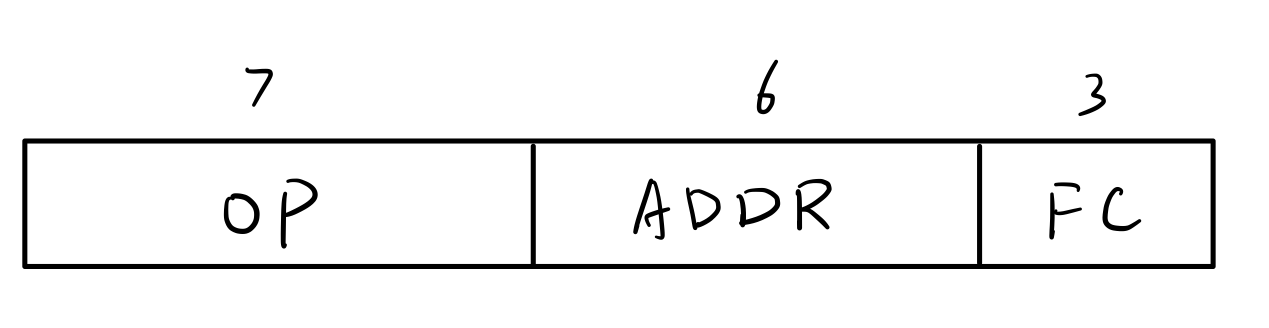
\includegraphics[width=5cm]{fig/7.16.png}
            \caption{题7.16}
            \label{fig:7_16}
        \end{figure}
        各字段作用: OP是指令的操作码字段, 为提供$108$种操作, 需要有$7$位以实现$2^7=128$种组合.
        ADDR是寻址地址, 用于不同的寻址. 使用补码.
        FC是寻址类型标志段, 为提供$6$种类型, 需要有$3$位以实现$2^3=8$种组合.

        \item 有$6$位地址, 最大范围是$2^6 = 64$, 单位为字 (16位).

        \item 一次间接寻址的寻址范围来自内存中一个字存储的地址, 最大范围是$2^{16} = 64\mathrm{K}$字. 多次间接寻址, 可每次移动 $-32\mathrm{K} \sim +32\mathrm{K} - 1$字, $n$次即可转移 $-32n\mathrm{K} \sim +32n\mathrm{K} - n$字, 范围是$64n\mathrm{K}-n+1$字.

        \item 因为有$6$位, 故为$-32 \sim 31$.

        \item $-32 \sim 31$.

        \item 立即寻址时间最短, 因为立即数可以直接访存, 不需要复杂寻址.
        
        间接寻址时间最长, 因为需要进行 (至少) 一次访存来寻址, 访存花时间长.
        
        随程序浮动, 使用相对寻址最合适, 因为这个操作数的结果会随着程序执行到的位置浮动, 是跟PC有关的.

        处理数组, 使用变址寻址最合适, 因为可以设定一个可变的位置来寻址, 如果一直访问一个数组的话就不需要改变这个寄存器.

        \item $4\mathrm{M} = 2^{22}$, 因此需要$22$位的地址, 而$22=16+6$, 需要将指令改成双字长的 (即添加16位地址), 如图\ref{fig:7_16_2}.
        \begin{figure}[!htbp]
            \centering
            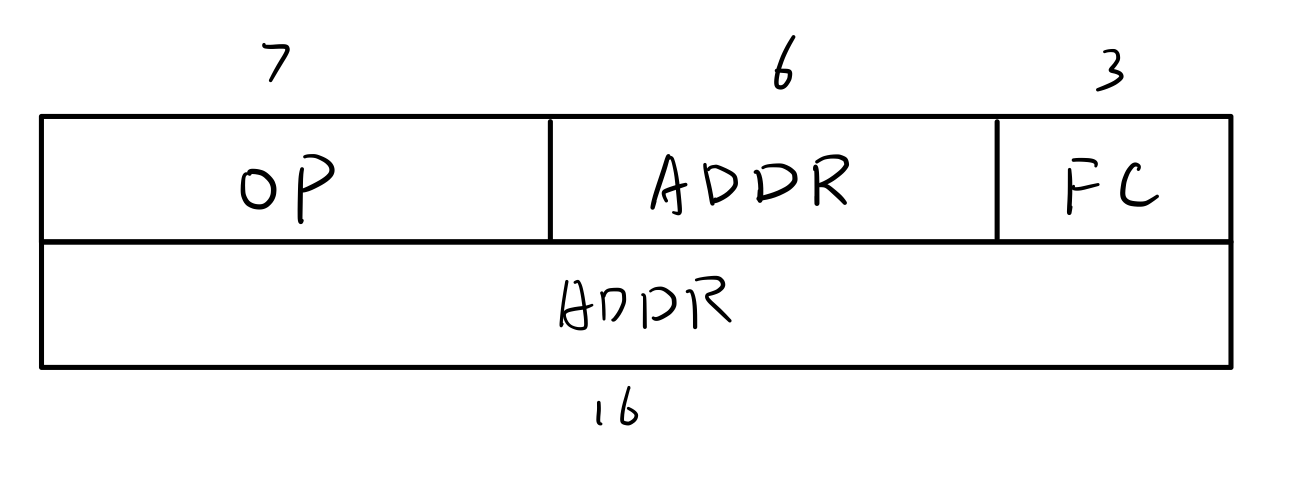
\includegraphics[width=5cm]{fig/7.16_2.png}
            \caption{题7.16}
            \label{fig:7_16_2}
        \end{figure}

        \item 按照如上所述的方式, 使用直接寻址即可实现. 
        \end{enumerate}
\end{solution}














\end{document}